\documentclass[a4paper, 12pt,oneside]{article} 
%\documentclass[a4paper, 12pt,oneside,draft]{article} 
\usepackage{preamble}
%--------------------- ACTUAL FILE ---------------------- %
\begin{document} 
%%%
	\begin{titlepage}
    \newcommand{\HRule}{\rule{\linewidth}{0.5mm}} % Defines a new command for the horizontal lines, change thickness here
    
    \center  % Center everything on the page
     
    %----------------------------------------------------------------------------------------
    %   HEADING SECTIONS
    %----------------------------------------------------------------------------------------

    \vspace{3cm}
    \textsc{\LARGE École polytechnique fédérale de Lausanne}\\[1.5cm] % Name of your university/college
    
    \textsc{\Large Regression Methods Project Report}\\[0.5cm] % Major heading such as course name
    \textsc{\large Coin-Data Regression Study}\\[0.5cm] % Minor heading such as course title
    
    %----------------------------------------------------------------------------------------
    %   TITLE SECTION
    %----------------------------------------------------------------------------------------
    
    \HRule \\[0.4cm] % line above and under the title
    
    
    % Title of your document
    
    \HRule \\[1.5cm]
     
    %----------------------------------------------------------------------------------------
    %   AUTHOR SECTION
    %----------------------------------------------------------------------------------------
    
    \begin{minipage}{0.4\textwidth}
    \begin{flushleft} \large
    
    \emph{Authors:}\\
    Tara \textsc{Fjellman}\\
    Rayan \textsc{Harfouche}\\
    
    
    
    
    \end{flushleft}
    \end{minipage}
    ~
    \begin{minipage}{0.4\textwidth}
    \begin{flushright} \large
    
    \emph{Professor:} \\
    Anthony \textsc{Davison}\\
    \end{flushright}
    \end{minipage}\\[10cm]
    %
    
    
    %----------------------------------------------------------------------------------------
    %   LOGO SECTION
    %----------------------------------------------------------------------------------------
    
    
\includegraphics[width=0.4\linewidth]{Logo-1 .pdf}\\[1cm] 
    % Include a department/university logo - this will require the graphicx package
     
    %----------------------------------------------------------------------------------------
    
    \vfill % Fill the rest of the page with whitespace
    
    \end{titlepage} 
	% Add titlepage
	\clearpage
	\tableofcontents
	\thispagestyle{empty}
	% Add table of contents
	\clearpage
	\pagenumbering{arabic}
	\setcounter{page}{1}
	\section*{Abstract}
		context of the original paper (with their claims). The paper that won the 2024 IgNobel Prize in Probability took a Bayesian approach to studying the statistics behind the coin-flipping process. Its main goal was to confirm a prediction made by a physical model of human coin tossing developed by Diaconis, Holmes, and Montgomery (DHM; 2007); i.e. that when people flip an ordinary coin, the probability of it landing on the same side it started is about 51\%. 
		It also revealed considerable between-people variation in the degree of this same-side bias, as well as its decrease as more coins were flipped. 

		The goal of this report is two fold. On the one side, we aim to investigate similar questions with a regression approach : 
		is there evidence for between-person, between-coin, or even person-coin pair differences ? To what extent does flipping experience affect the observed same-side bias ?
		In addition, we also investigate the differences between GLM and WLS approaches; as well as muscle memory effects (through outcomes of recent flips). 
	\section{Introduction}
		Before diving into the analysis, we provide a brief overview of the datasets main features and the models we consider. Our exploratory analysis is available as a Jupyter notebook, and provides more detail. 

		The dataset is composed of throws from 48 people using 44 coins in total. Given the study did not impose strict guidelines for coins to be used, the design is heavily unbalanced. Eighteen coins have only been thrown by a single person, while some of them have been thrown by more than 20 people. Also, more than half the people have only flipped 5 or less different coins, while someone threw 11 different ones. As for the the person-coin pairs, most have fewer or equal to 1000 throws, while some have around 10000 ones. This severe unbalance must be kept in mind during the study, given it can pose challenges during model interpretation. 

		After plotting the same-side rates across people, coin and person-coin combinations, we deemed it relevant to investigate models considering both person and coin as covariates, as well as individual person-coin pairs. Following the advice given on the project statement, we also branched our analysis in Binomial-response GLM and WLS approaches. 

		Motivated by impacts of muscle-memory on the flipping, we additionally investigated aspects such as time-varying same-side rates and memory between successive throws.
	\section{Analysis}
		\subsection{Model Comparison}
			In this section, we introduce and compare different models for the same side success rate. 

			Some GLMs with binomial responses and some WLS ones based on the ... approximation.
			
			Should explain no a priori response transformation ...
			
			For each, the considered formulas in terms of the covariates are:
			\begin{itemize}
				\item \texttt{1}, corresponding to a constant model.
				\item \texttt{1+C(person)}, corresponding to a model with the person as a covariate.
				\item \texttt{1+C(person)+C(coin)}, corresponding to a model with the person and the coin as covariates.
				\item \texttt{1+C(person)+C(coin)+C(person):C(coin)}, corresponding to a model with the person, the coin, and the interaction between the person and the coin as covariates.
			\end{itemize}
			* model 4 could seem redundant due to nesting-main effect, but we ....
			*  

			Should explain why eliminated some covariates ...
			\subsubsection{Tools For Selection}
			\begin{itemize}
				\item when to use AIC vs LRT ?
				\item citing a few things about LRT not miting overfitting 
				\item 
			\end{itemize}
			\subsubsection{WLS Approach}

			\subsubsection{GLM Approach}
			\lipsum[1]
			\begin{table}[htb]
				\centering
				\caption{Model comparison for different models.}
				\label{tab:model-comparison}
				\begin{tabular}{lccc}
				\toprule
				Model & Deviance & AIC & Model DF \\
				\midrule
				\texttt{1} & 3943.48 & 173.97 & 0 \\
				\texttt{1+C(person)} & 3677.51 & 0.00 & 46 \\
				\texttt{1+C(person)+C(coin)} & 3611.12 & 17.61 & 88 \\
				\bottomrule
				\end{tabular}
			\end{table}
			\lipsum[1]
			\begin{figure}[htb]
				\centering
				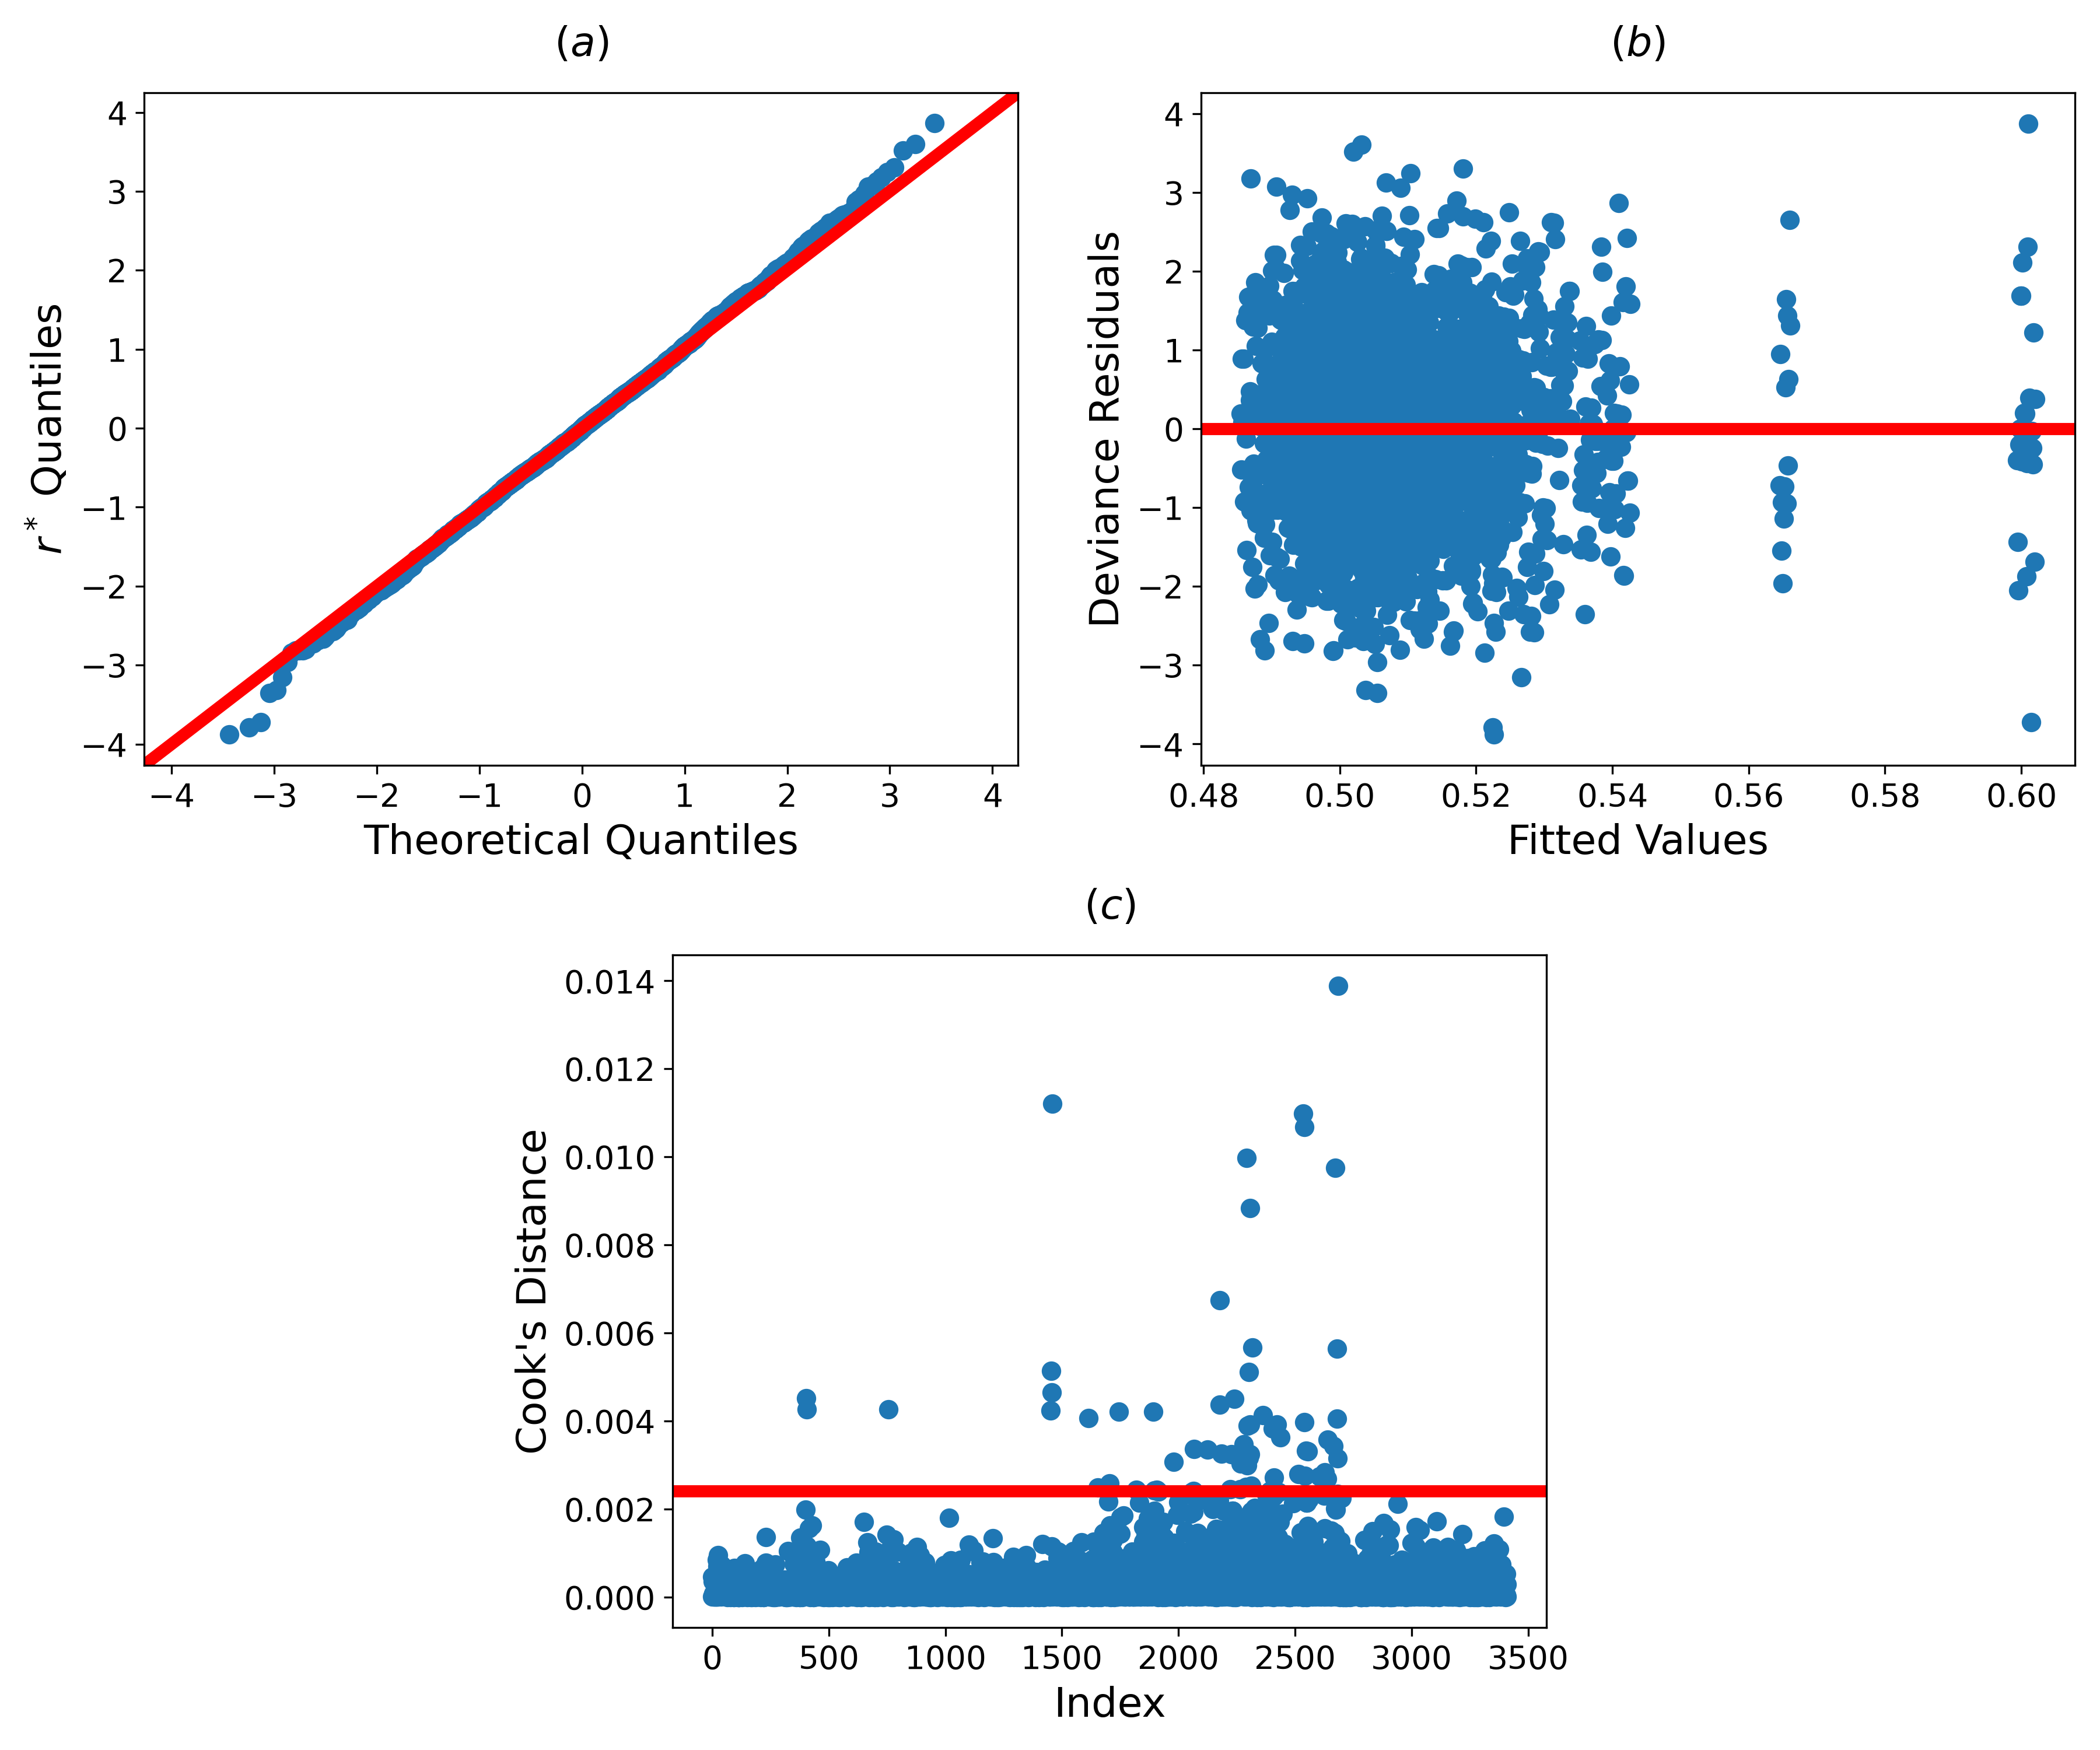
\includegraphics[width=0.85\textwidth]{GLM_diagnostics.png}
				\caption{Diagnostics for the selected GLM model. (a).}
				\label{fig:glm-diagnostic}
			\end{figure}
			\lipsum[1]
			\begin{table}[htb]
				\centering
				\caption{Likelihood ratio tests between models.}
				\label{tab:llr-comparison}
				\begin{tabular}{llc}
				\toprule
				Tested model & Restricted model & $p$-value \\
				\midrule
				\texttt{1+C(person)} & \texttt{1} & 0.00e+00 \\
				\texttt{1+C(person)+C(coin)} & \texttt{1+C(person)} & 9.61e-03 \\
				\bottomrule
				\end{tabular}
			\end{table}
		\subsection{Unusual Observations}
		\begin{figure}[htb]
			\centering
			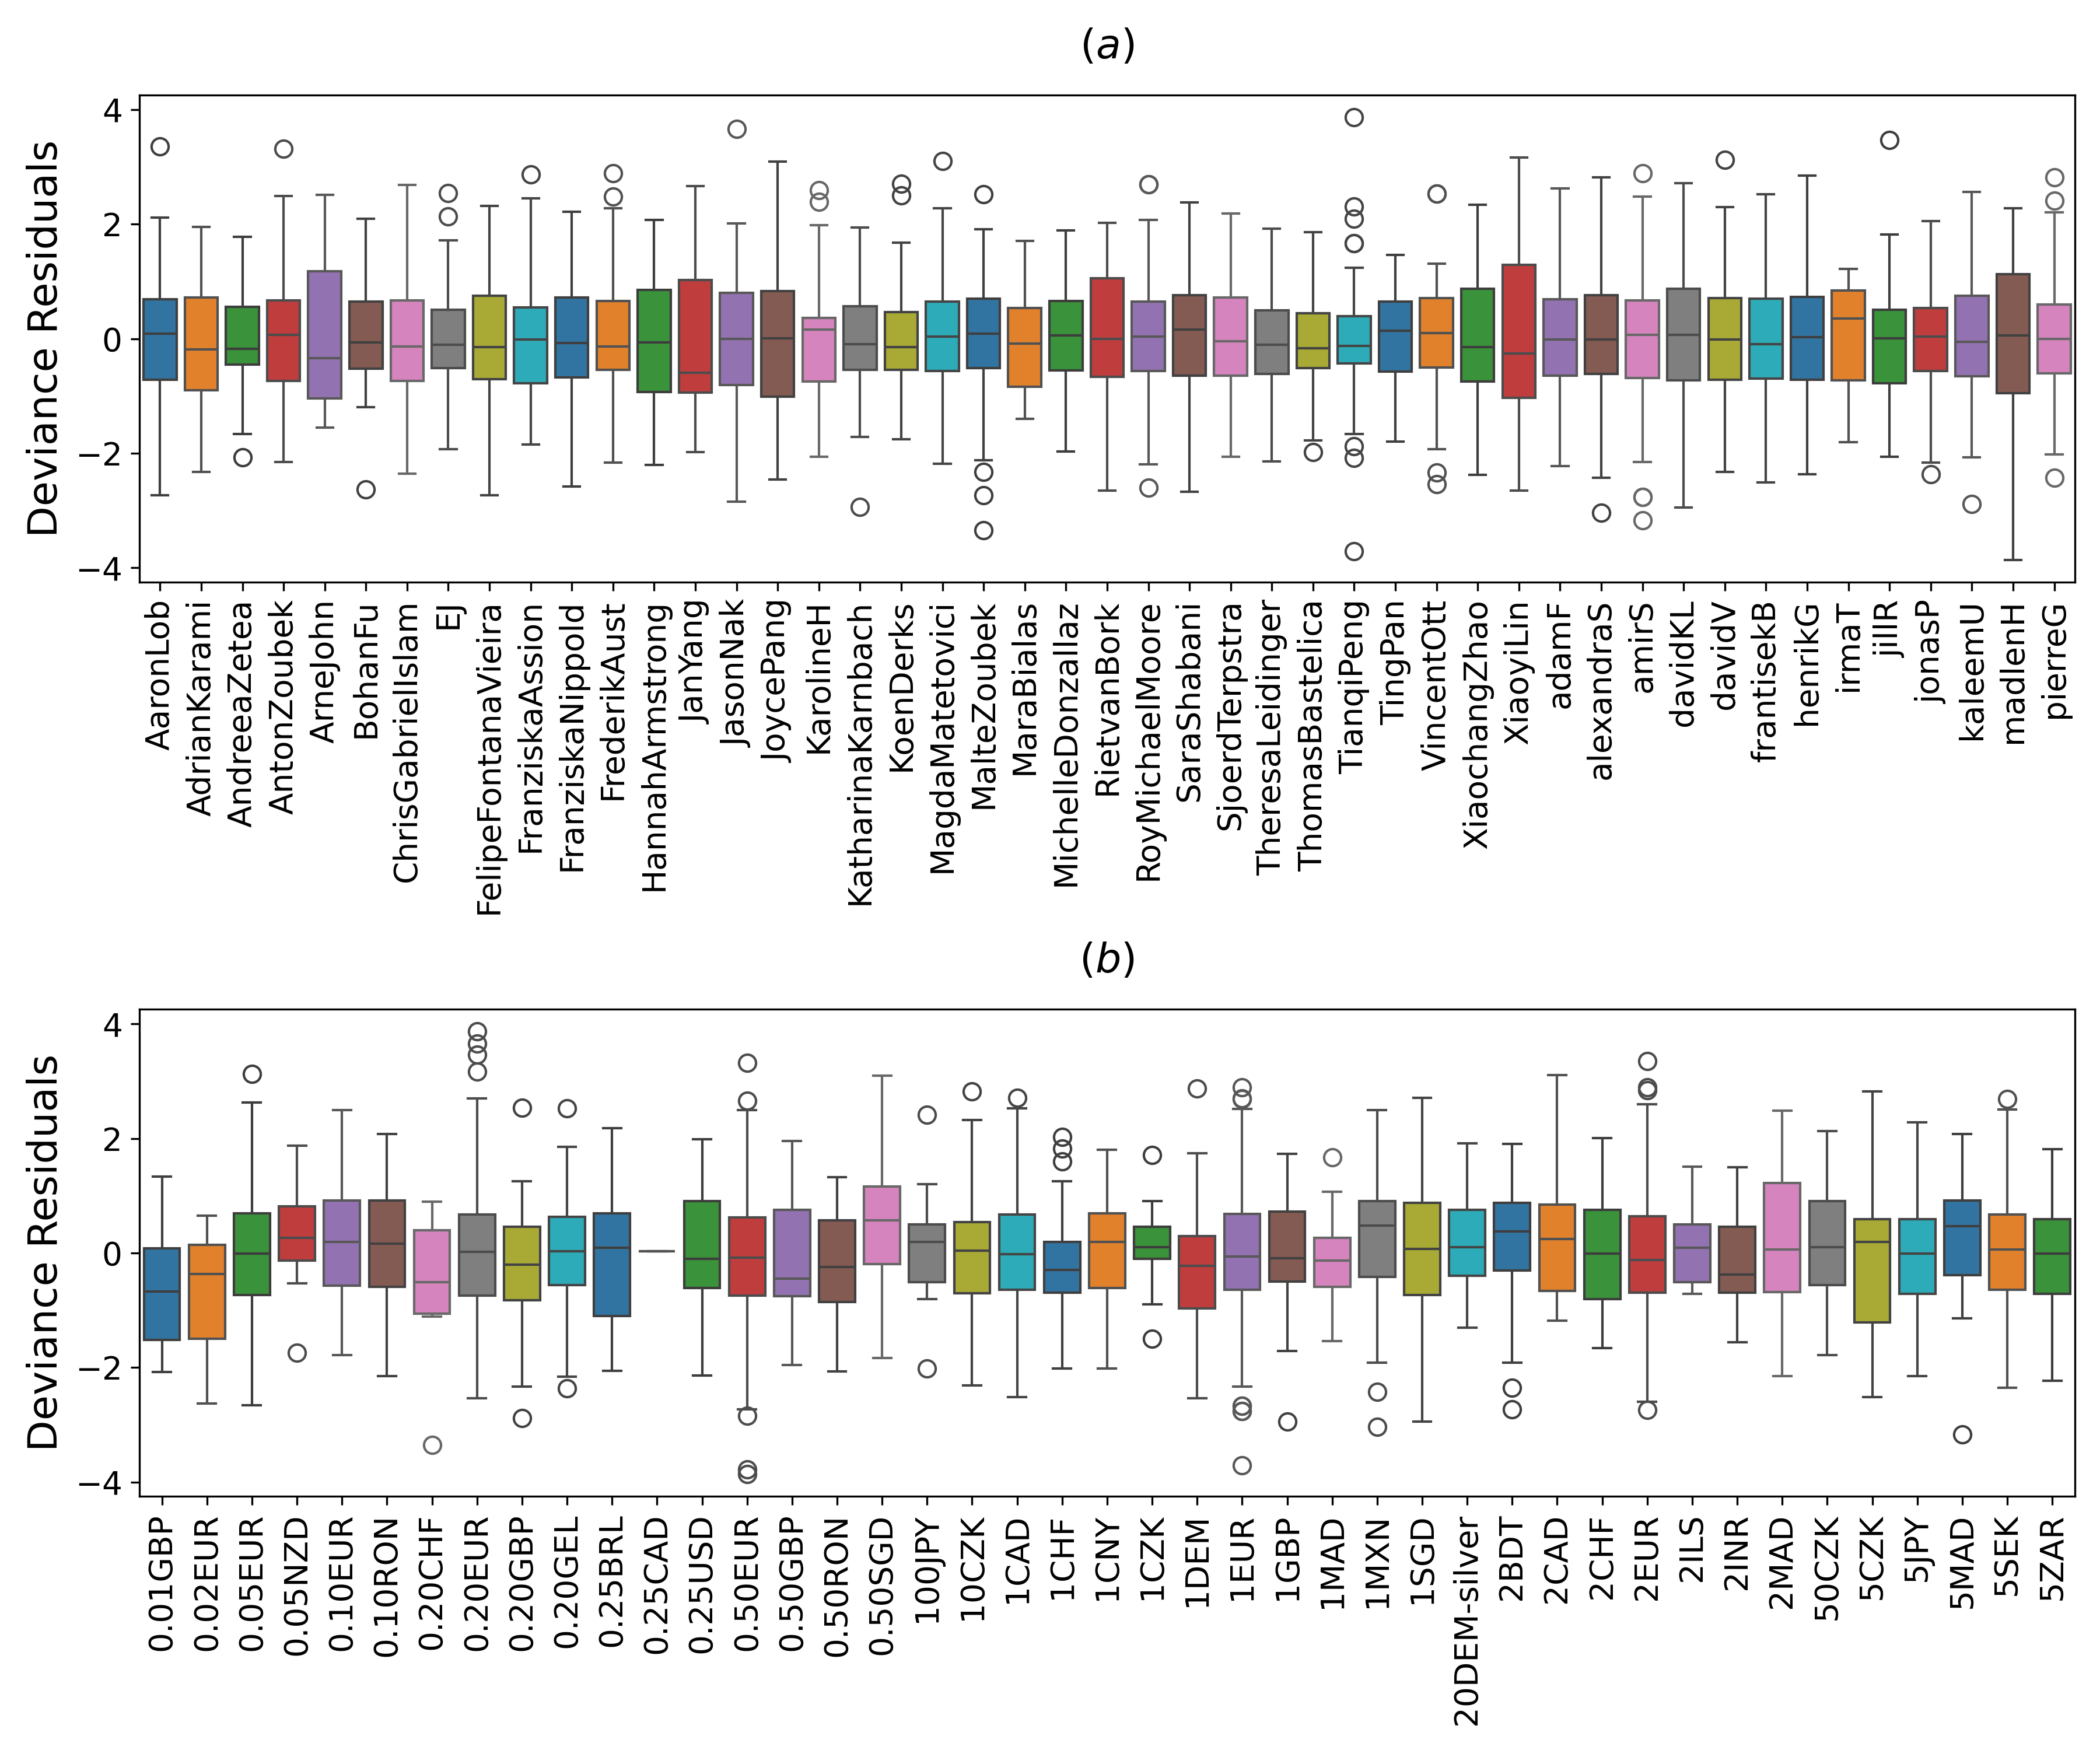
\includegraphics[width=0.85\textwidth]{dev_resid_vs_covariates.png}
			\caption{Dev-resid as a function of (a) person and (b) coin.}
			\label{fig:dev-resid-vs-covariates}
		\end{figure}

		\subsection{Zoom on Learning Effects}
		\begin{itemize}
			\item bias comes from start
			\item amount of bias (considerable)
			\item wobble interpretation (consistent with physical model, citing the paper)
		\end{itemize}
		\lipsum[1]
		\begin{figure}[htb]
			\centering
			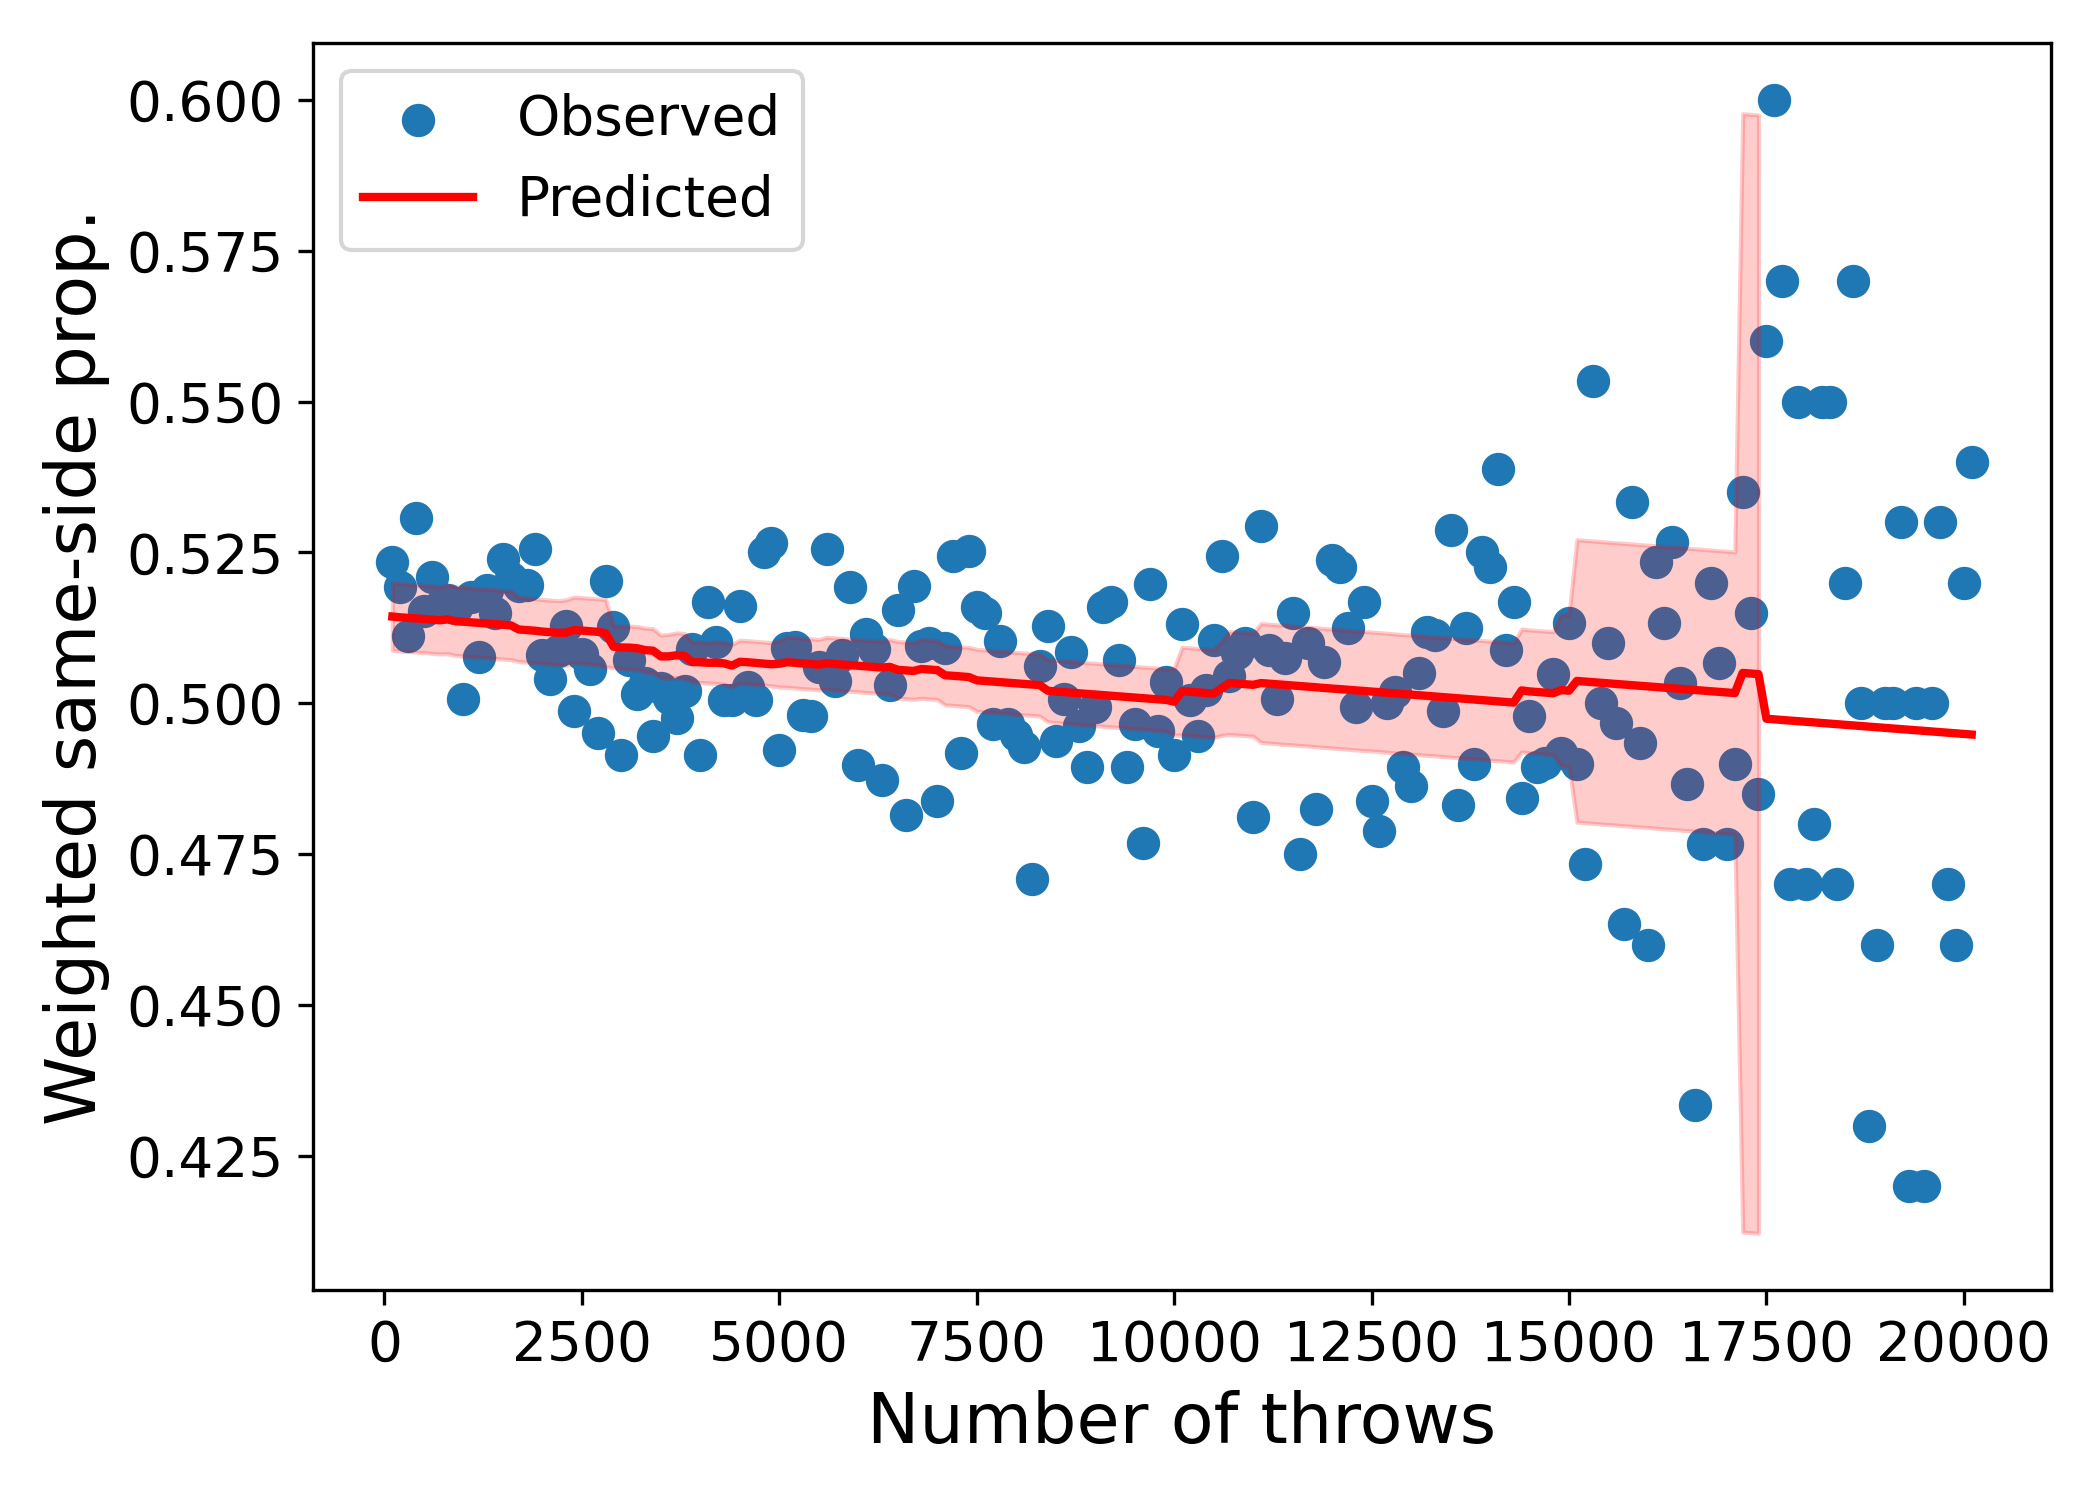
\includegraphics[width=0.5\textwidth]{learning_effects.png}
			\caption{Learning effects.}
			\label{fig:learning-effects}
		\end{figure}
		\subsection{Memory Effects}
		In this section we shift our focus to memory effects. We do so motivated by the fact that we deem it probable a priori that successive throws are more similar to each other than randomly selected ones. Indeed, one could imagine that after two same-side throws, the next could end being a same-side one two with a probability higher than the base rate. 
		
		To test this we start by considering the data consisting of individual throw outcomes. To this, we add columns corresponding to 
		\begin{itemize}
			\item same-side indicator variables,
			\item same-side indicator variables for the penultimate throw,
			\item same-side indicator variables for the antepenultimate throw.
		\end{itemize}
		To deal with the boundary effects between sequences of flips, we removed the two first entries of each sequence. 
		%To speed up the computations
		
		We then define the models 
		\begin{itemize}
			\item \texttt{1}, same-side indicator variables,
			\item \texttt{1+hop1\_mem}, same-side indicator variables for the penultimate throw,
			\item \texttt{1+hop1\_mem+hop2\_mem}, same-side indicator variables for the antepenultimate throw.
		\end{itemize}
		and carry out an analysis of deviance. The results associated are found in \ref{tab:memory-model-comparison}. Given the uni-directionality of these results, no further analysis was made.  
		\begin{table}[htb]
			\centering
			\caption{Model comparison for models including : no memory, 1-hop memory and 2-hop memory.}
			\label{tab:memory-model-comparison}
			\begin{tabular}{lccc}
			\toprule
			Model & Deviance & AIC & Model DF \\
			\midrule
			\texttt{1} & 474381.54 & 0.00 & 0 \\
			\texttt{1+hop1\_mem} & 474380.73 & 1.19 & 1 \\
			\texttt{1+hop1\_mem+hop2\_mem} & 474380.53 & 2.98 & 2 \\
			\bottomrule
			\end{tabular}
		\end{table}
	\section{Discussion}


	\subsection{Memory effects}
	Looking at \ref{tab:memory-model-comparison}, we see there is no support in favour of memory effects relative to the constant model. The deviance decreases by around .8 due to the introduction of the penultimate throw memory and only a further .2 when including memory of the antepenultimate throw. Another factor that shows this is the increase by $>$1 and $\approx 3$ respectively in AIC compared to the constant model.
	The fact that memory about antepenultimate outcome seems to matter even less than memory about the penultimate outcome does make nonetheless intuitive sense. 

	This (non-) finding can in itself be regarded as reassuring in a way. Specifically, it might contribute to rule out concerns of the authors of the original paper regarding the potential same-side bias induced by participants knowing about the goal of the study. Indeed it seems far-fetched that someone could bias their throws without relying on muscle memory. 
	\section{Conclusion}
	\section*{Acknowledgements}
	\section*{References}
	%\appendix
	%	\section{Runtime Estimation}\label{appendix:runtime_estimation}
%%%
\end{document} 